\chapter{Influence of fluid dynamics of the system on the extracted power}

\section{Introduction}

This chapter contains the results and discussion relating to the third objective of this thesis. As discussed in chapter \ref{chap:lit-review} the induced force $F_y$ of the system is a result of the top and bottom of the shear layer behaviour of the system. The current published work shows that the afterbody of the system has a significant influence on the galloping response. In this chapter, the influence of shear layer behaviour and hence, the influence of the afterbody on mean extracted power is discussed.

Here, the influence of shear layer on the mean power is studied by introducing a cross section which is a hybrid of a square and a triangle. Data are analysed the cross section is transformed gradually by manipulating the ratio of two length scales.

The stationary forcing data is presented for each cross section followed by the QSS power curves. Based on the QSS power data, an optimum cross section for power extraction is identified. Next, the underpinning reason for the negative portion of certain $C_y$ curves is discussed through surface pressure and flow velocity data. Following this, a reasoning for the discrepancy between QSS and DNS mean power at the optimum power cross section is discussed.       

A final summary is presented explaining the influence of the shear layer on mean power output and the preliminary design considerations to optimise the fluid mechanics to obtain an optimum power output. 


\section{Influence of the shear layers}

As highlighted in section \ref{subsec:fluid_mechanics_of_galloping} the afterbody of the cross section has a significant influence on galloping. This is because of the shear layer need to interact with the afterbody after separation at the leading edge. 


The $C_y$ vs $\alpha$ curve increases reaches a maximum and reduces as the induce angle is increased. The maximum of the induced lift occurs when the separated  shear layer (at the leading edge) closer to the surface of the body reattaches at the trailing edge. Therefore, by delaying the reattachment the point where the maximum lift occurs can be shifted towards a higher induced angle which leads to a higher induced velocity. As shown in equation \ref{eqn:power_alt} higher velocity leads to higher power output. In order to test this hypothesis the shear layer reattachment was reduced by gradually tapering off the top and bottom sides of the square cross section as sown in figure \ref{fig:hybrid_section}. The $\ratio$ was changed gradually from 1 to zero at increments of 0.25 where 1 being the square cross section and 0 being an isosceles triangle.    

\begin{figure}
\setlength{\unitlength}{\textwidth}

  \begin{picture}(1,0.23)(0,0.74)
    
  \put(0.2,0.76){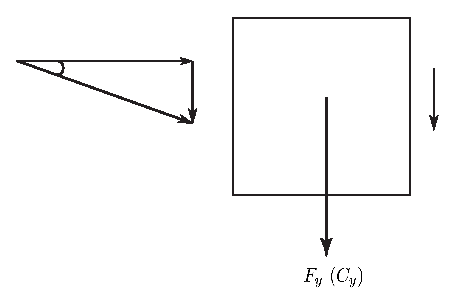
\includegraphics[width=0.5\unitlength]{../FnP/gnuplot/setup-1.eps}}         
      
      
   
 	\put(0.315,0.93){$U$}
 	\put(0.3,0.84){$U_i$}
    \put(0.42,0.88){$\dot{y}$}
    \put(0.28,0.895){ $\theta$}
    \put(0.7,0.87){\small $(+)$}
      	

 	
 	 

     

  \end{picture}

 \caption{Induced angle of attack on the square prism due to the resultant of free-stream velocity of the fluid and transverse velocity of the body.}
    \label{fig:setup_1}
\end{figure}


\begin{table}[ht]

\begin{center}
\setlength{\unitlength}{\textwidth}

\begin{tabular}{c c c c c} % centered columns (4 columns)
\hline\hline %inserts double horizontal lines
\\[0.2ex]
Case & $a_1$ & $a_3$ & $a_5$ & $a_7$ \\ [0.8ex] % inserts table 
%heading
\hline 
\\[0.8ex]% inserts single horizontal line
Re=200 & 2.32 & 197.8 & 4301.7 & 30311.9 \\[0.8ex]% inserting body of the table
Re=22300 & 2.69 & 168 & 1670 & 59900 \\ [1ex] % [1ex] adds vertical space
\hline %inserts single line
\end{tabular}

\caption{Coefficient values used in the 7th order interpolation polynomial for high ($Re=22300$) and low ($Re=200$) Reynolds numbers. These data are used as input data to calculate the right-hand side of Eq. \ref{final_equation_motion} throughout this study.}
 
\label{table:cy-coefficients} % is used to refer this table in the text
\end{center}
\end{table}


\begin{figure}
  \setlength{\unitlength}{\textwidth}

  \begin{picture}(1,0.75)(0,0)
    % % %90
      % % % Parkinson Data 
      \put(0.035,0.5){\includegraphics[width=0.5\unitlength]{./FnP/lift_curve_sq.eps}}
      \put(0.495,0.5){\includegraphics[width=0.5\unitlength]{./FnP/lift_curve_075.eps}}
      \put(0.035,0.27){\includegraphics[width=0.5\unitlength]{./FnP/lift_curve_05.eps}}
      \put(0.495,0.27){\includegraphics[width=0.5\unitlength]{./FnP/lift_curve_025.eps}}
      \put(0.3,0.0){\includegraphics[width=0.5\unitlength]{./FnP/lift_curve_tri.eps}}
      
      
   
      
      
%      \put(0.23,0.00){ $\displaystyle\frac{c}{\rho\mathcal{A}U}$}
%      \put(0.73,0.00){ $\displaystyle\frac{c}{\rho\mathcal{A}U}$}

      \put(0.3,0.26){$\theta$}
      \put(0.76,0.26){$\theta$}
      \put(0.56,-0.01){$\theta$}
      
      \put(0.01,0.405){$\displaystyle C_y$}
       \put(0.01,0.65){$\displaystyle C_y$}
      \put(0.3,0.14){$\displaystyle C_y$}
      
      \put(0.106,0.705){\small(a)}
      \put(0.565,0.705){\small(b)}
      \put(0.106,0.475){\small(c)}
      \put(0.565,0.475){\small(d)}
      \put(0.37,0.207){\small(e)}
      

  \end{picture}

  \caption{Induced lift coefficient $C_y$ at different angles for selected cross sections. Data presented for cross sections, (a) square, (b) $\ratio=0.75$, (c) $\ratio=0.5$, (d) $\ratio=0.25$ and (e) triangle.}
  \label{fig:lift_curves}
\end{figure}

% !TeX spellcheck = en_GB
\begin{figure}[!htb]
  \setlength{\unitlength}{\textwidth}

        \begin{picture}(1,0.4)(-0.02,0)

 
      
      \put(0.08,0.02){\includegraphics[width=0.75\unitlength]{./chapter-cross-sections/fnp/mean_power_hyb.eps}}

      \put(0.46,0.00){\massdamp}
      
      
     
       \put(0.03,0.235){$\displaystyle\frac{P_{m}}{\rho \mathcal{A}U^3 }$}
      

      %\put(0.095,0.218){\small(a)}
      %\put(0.565,0.218){\small(b)}
      
    \end{picture}

  \caption{Dimensionless mean power obtained using QSS model as a function of \massdamp. Data presented for five selected cross sections, square ($\triangle$), $\ratio=0.75$ (+), $\ratio=0.5$ (\ding{117}), $\ratio=0.25$ ($\times$) and triangle (\ding{108}) at $\reynoldsnumber=200$, $\massstiff=100$.}
    \label{fig:power_curves}
\end{figure}

 %vspace{10cm}

\begin{figure}
  \setlength{\unitlength}{\textwidth}

        \begin{picture}(1,1.1)(0,0.35)

      % % % Parkinson Data 
      \put(0.1,1.1){\includegraphics[width=0.75\unitlength]{./chapter-cross-sections/fnp/surf-pres-tri-4.eps}}
      \put(0.1,0.737){\includegraphics[width=0.75\unitlength]{./chapter-cross-sections/fnp/surf-pres-tri-16.eps}}
      \put(0.1,0.38){\includegraphics[width=0.75\unitlength]{./chapter-cross-sections/fnp/surf-pres-tri-21.eps}}
     
      
      



%      
    \put(0.21,1.41){\small(a)}
     \put(0.21,1.05){\small(b)}
     \put(0.21,0.69){\small(c)}
\put(0.1,0.95){$\displaystyle P_{s}$}
\put(0.1,1.3){$\displaystyle P_{s}$}
\put(0.1,0.56){$\displaystyle P_{s}$}
\put(0.26,0.35){Relative destance from the leading edge}

      
    \end{picture}

    \caption{Surface pressure of top (\ding{83}) and bottom (\ding{117})  surfaces of the static triangular cross section at (a) $\theta=4^\circ$, (b) $\theta=16^\circ$ \ and (c) $\theta=21^\circ$ A clear pressure difference is visible between the surfaces. The top surface comparatively has more negative pressure where a lift is created which results in a negative $C_y$ at $4^\circ$ and reduces as $\theta$ \ is increased, while the vice versa occurs at the top surface.}
    \label{fig:surf_pres}
\end{figure}

 %vspace{10cm}

\begin{figure}
  \setlength{\unitlength}{\textwidth}

        \begin{picture}(1,1.1)(0,0.35)

      % % % Parkinson Data 
      \put(0.1,1.1){\includegraphics[width=0.75\unitlength]{./chapter-cross-sections/fnp/vel_prof-tri-4.eps}}
      \put(0.1,0.737){\includegraphics[width=0.75\unitlength]{./chapter-cross-sections/fnp/vel_prof-tri-16.eps}}
      \put(0.1,0.38){\includegraphics[width=0.75\unitlength]{./chapter-cross-sections/fnp/vel_prof-tri-21.eps}}
     
      
      



%      
    \put(0.21,1.41){\small(a)}
     \put(0.21,1.05){\small(b)}
     \put(0.21,0.69){\small(c)}
\put(0.1,0.95){$\displaystyle V_m$}
\put(0.1,1.3){$\displaystyle V_m$}
\put(0.1,0.56){$\displaystyle V_m$}
\put(0.34,0.35){Distance from the leading edge}

      
    \end{picture}

    \caption{Velocity magnitudes of the flow along a line parallel to the front surface spreading towards top (\solidrule) and bottom (\dashedrule) boundaries (figure \ref{fig:tri-sketch}). These two lines (for the top and bottom surfaces) start from the top and bottom leading edges of the triangular cross section. Data present (a) $\alpha=4^\circ$, (b) $\alpha=16^\circ$ \ and (c) $\alpha=21^\circ$.}
    \label{fig:surf_pres}
\end{figure}

 %vspace{10cm}

% !TeX spellcheck = en_GB
\begin{figure}[!htb]
  \setlength{\unitlength}{\textwidth}

        \begin{picture}(1,0.4)(-0.02,0)

 
      
      \put(0.08,0.02){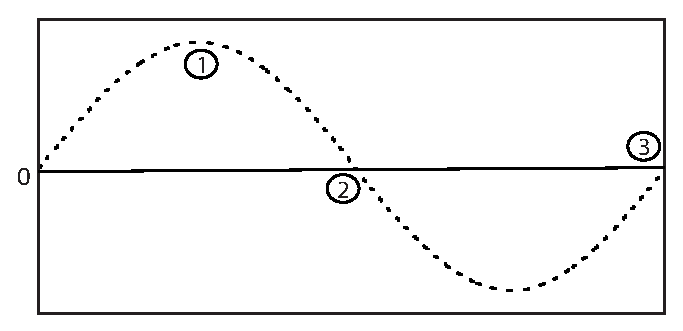
\includegraphics[width=0.75\unitlength]{./chapter-cross-sections/fnp/fsi_flow_sketch.eps}}

      %\put(0.46,0.00){\massdamp}
      
      
     
       %\put(0.03,0.235){$\displaystyle\frac{P_{m}}{\rho \mathcal{A}U^3 }$}
      

      %\put(0.095,0.218){\small(a)}
      %\put(0.565,0.218){\small(b)}
      
    \end{picture}

  \caption{}
    \label{fig:power_curves}
\end{figure}

 %vspace{10cm}

\begin{figure}[htbp]
  \setlength{\unitlength}{\textwidth}

  \begin{picture}(1,1.19)(0,0)
    % % %90
      % % % Parkinson Data 
      \put(0.005,0.8){\includegraphics[width=0.4\unitlength]{./chapter-cross-sections/fnp/{fsi-0.25-1}.eps}}
      \put(0.005,0.4){\includegraphics[width=0.4\unitlength]{./chapter-cross-sections/fnp/{fsi-0.25-2}.eps}}
      \put(0.005,0.0){\includegraphics[width=0.4\unitlength]{./chapter-cross-sections/fnp/{fsi-0.25-3}.eps}}

      
      
      \put(0.505,0.8){\includegraphics[width=0.4\unitlength]{./chapter-cross-sections/fnp/{qss-0.25-1}.eps}}
      \put(0.505,0.4){\includegraphics[width=0.4\unitlength]{./chapter-cross-sections/fnp/{qss-0.25-3}.eps}}
      \put(0.505,0.0){\includegraphics[width=0.4\unitlength]{./chapter-cross-sections/fnp/{qss-0.25-3}.eps}} 
      
      
%      \put(0.23,0.00){ $\displaystyle\frac{c}{\rho\mathcal{A}U}$}
%      \put(0.73,0.00){ $\displaystyle\frac{c}{\rho\mathcal{A}U}$}


      
      \put(0.01,1.125){\small(a)}
      \put(0.510,1.125){\small(b)}
      \put(0.01,0.725){\small(c)}
      \put(0.510,0.725){\small(d)}
      \put(0.01,0.33){\small(e)}
      \put(0.510,0.33){\small(f)}
      
   
   
      

  \end{picture}

  \caption{Time averaged stream functions of stationary and oscillating flow-fields of the hybrid cross section ($\ratio=0.25$), averaged over a vortex shedding cycle. (a), (c) and (e) are the averaged stream functions of the oscillating case at $\frac{tU}{D}=2295.763$ (point 1), $\frac{tU}{D}=2305.897$ (point 2) and $\frac{tU}{D}=2325.870$ (point 3) . (b), (d) and (f) are the stream functions of the flow field of the stationary body corresponding to the induced angles of (a), (c) and (e).}  
  \label{fig:flow_field_FSI}
\end{figure}

